\documentclass[border=0.2cm]{standalone}

% Required packages
\usepackage{tikz}
\usetikzlibrary{shapes,positioning}

\begin{document}

	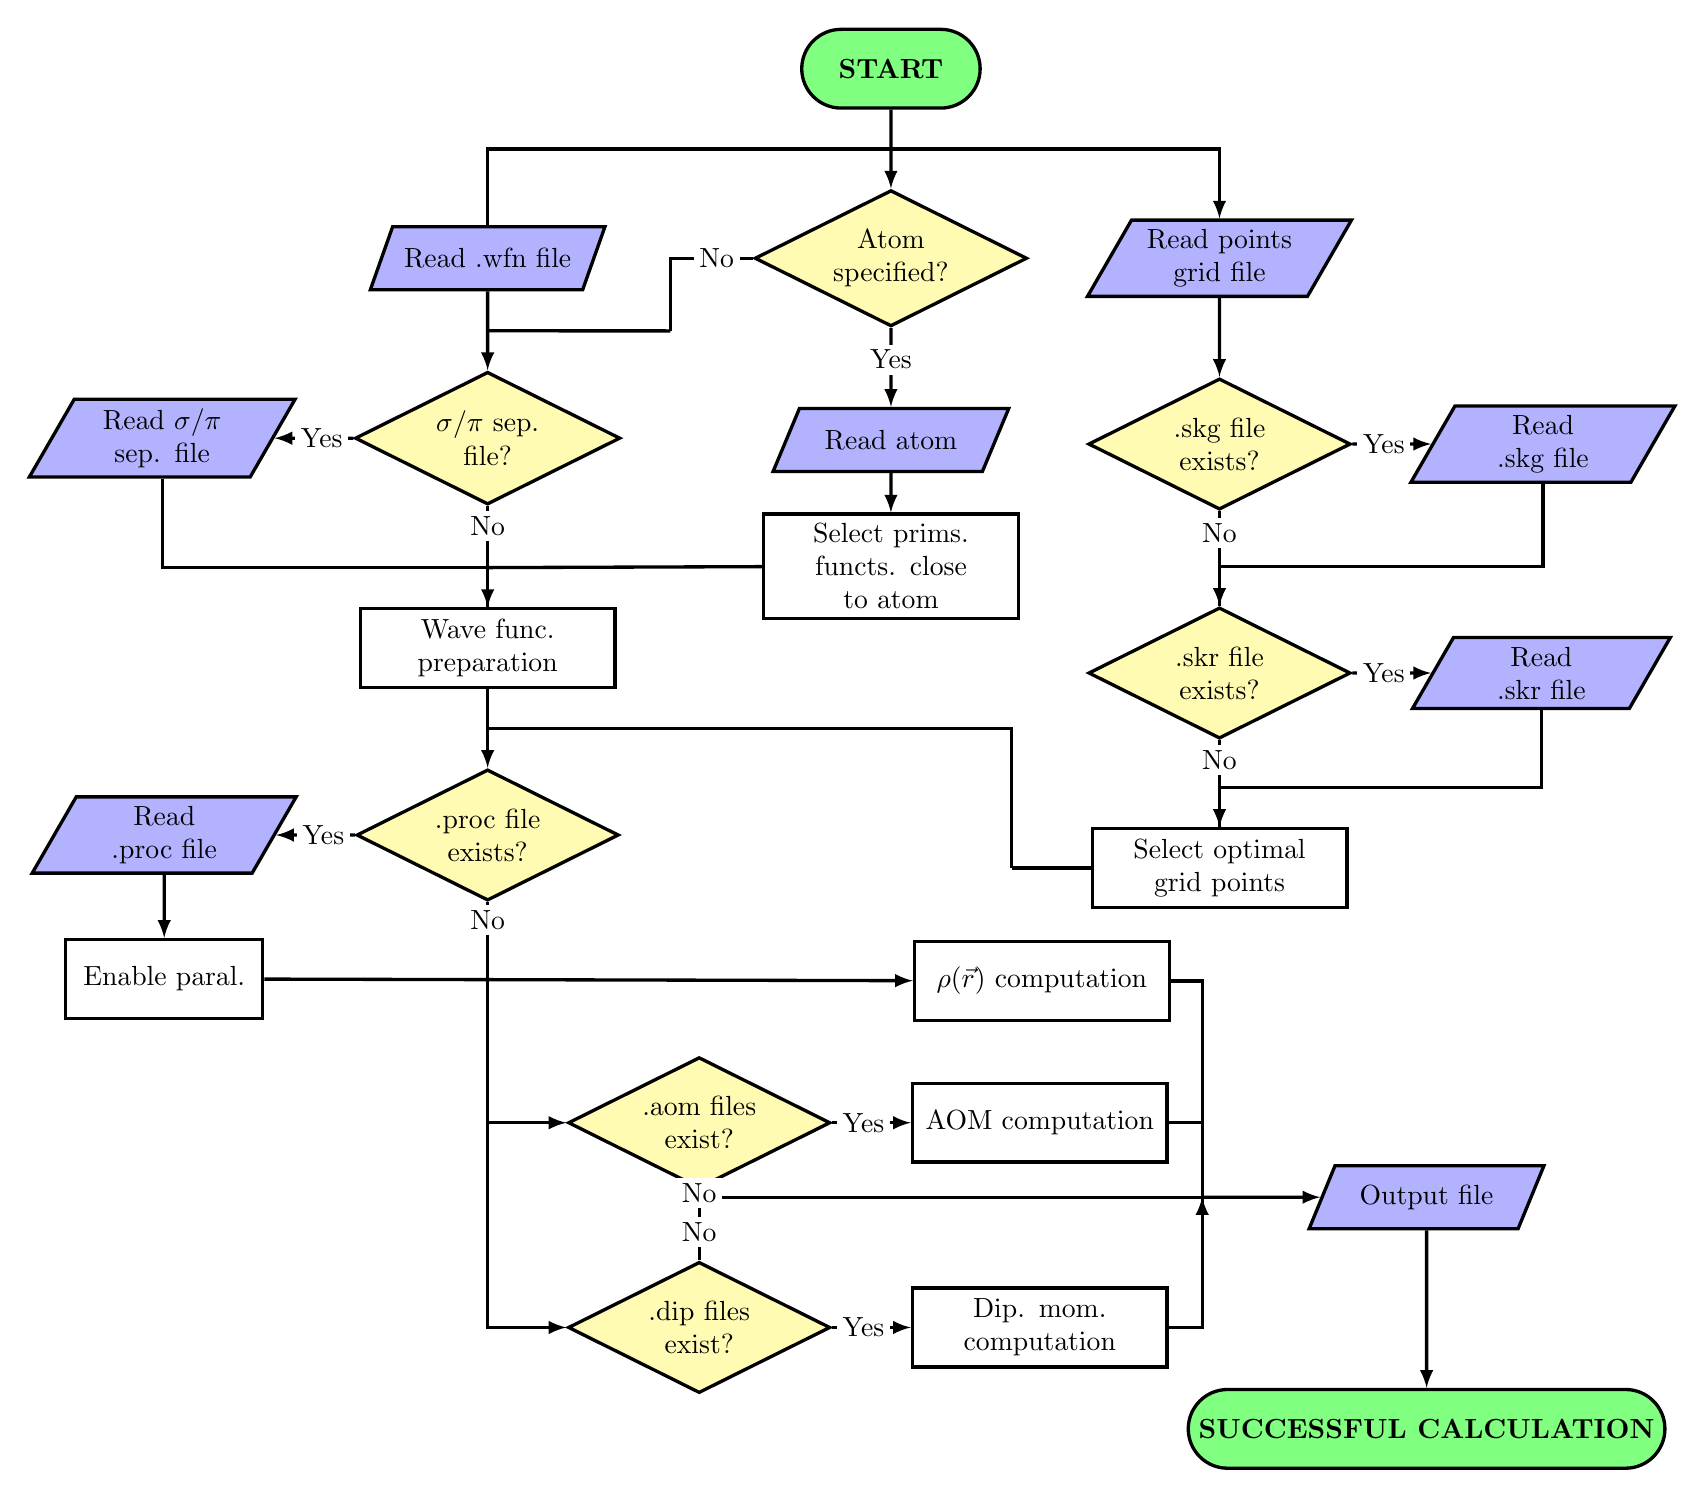
\begin{tikzpicture}[font=\normalsize,very thick,align=center]

		% Start block
		\node[
			draw,
			fill=green!50,
			rounded rectangle,
			minimum width=2.5cm,
			minimum height=1cm
		] (start) {\textbf{START}};

		\node[coordinate,below=.5cm of start] (ghoststart) {};

		% Third argument?
		\node[
			draw,
			diamond,
			aspect=2,
			minimum width=2.cm,
			text width=3cm,
			text centered,
			inner sep=0,
			fill=yellow!30,
			text width=2cm,
			below=.5cm of ghoststart
		] (thirdarg) {Atom specified?};

		\node[coordinate,below left=of thirdarg] (ghostthird) at (-1.8cm,-2.33cm) {};

		% Read wfn file
		\node[
			draw,
			trapezium,
			trapezium left angle = 60,
			trapezium right angle = 120,
			trapezium stretches,
			minimum width=3.cm,
			minimum height=.8cm,
			fill=blue!30,
			left=2cm of thirdarg
		] (readwfn) {Read .wfn file};

		\node[coordinate,below=.5cm of readwfn] (ghostwfn) {};

		% Read grid file
		\node[
			draw,
			trapezium,
			trapezium left angle = 60,
			trapezium right angle = 120,
			trapezium stretches,
			minimum width=3.cm,
			minimum height=.8cm,
			text width=2cm,
			fill=blue!30,
			right=of thirdarg
		] (readgrid) {Read points grid file};

		% Read atom grid is centered on
		\node[
			draw,
			trapezium,
			trapezium left angle = 60,
			trapezium right angle = 120,
			trapezium stretches,
			minimum width=3.cm,
			minimum height=.8cm,
			fill=blue!30,
			below=of thirdarg
		] (readatom) {Read atom};

		% Read atom grid is centered on
		\node[
			draw,
			minimum width=2.5cm,
			minimum height=1cm,
			text width=3cm,
			below=.5cm of readatom
		] (skipprim) {Select prims. functs. close to atom};

		% .sg file exists?
		\node[
			draw,
			diamond,
			aspect=2,
			minimum width=2.cm,
			text width=2cm,
			text centered,
			inner sep=0,
			fill=yellow!30,
			below=.5cm of ghostwfn
		] (sigpi) {$\sigma$/$\pi$ sep. file?};

		% Read .sg file
		\node[
			draw,
			trapezium,
			trapezium left angle = 60,
			trapezium right angle = 120,
			trapezium stretches,
			minimum width=3.cm,
			minimum height=.8cm,
			fill=blue!30,
			text width=2cm,
			left=of sigpi
		] (sgread) {Read $\sigma$/$\pi$ sep. file};

		\node[coordinate,below=.78cm of sigpi] (ghostsigpi) {};

		% wf user settings
		\node[
			draw,
			minimum width=2.5cm,
			minimum height=1cm,
			text width=3cm,
			below=.5cm of ghostsigpi
		] (wfword) {Wave func. preparation};

		\node[coordinate,below=.5cm of wfword] (ghostwfword) {};

		% .skg file?
		\node[
			draw,
			diamond,
			aspect=2,
			minimum width=2.cm,
			text width=3cm,
			text centered,
			inner sep=0,
			fill=yellow!30,
			text width=2cm,
			below=of readgrid
		] (skg) {.skg file exists?};

		% Read .skg file
		\node[
			draw,
			trapezium,
			trapezium left angle = 60,
			trapezium right angle = 120,
			trapezium stretches,
			minimum width=3.cm,
			minimum height=.8cm,
			fill=blue!30,
			text width=2cm,
			right=of skg
		] (readskg) {Read .skg file};

		\node[coordinate,below=.7cm of skg] (ghostskg) {};

		% .skr file?
		\node[
			draw,
			diamond,
			aspect=2,
			minimum width=2.cm,
			text width=2cm,
			text centered,
			inner sep=0,
			fill=yellow!30,
			below=.5cm of ghostskg
		] (skr) {.skr file exists?};

		% Read .skg file
		\node[
			draw,
			trapezium,
			trapezium left angle = 60,
			trapezium right angle = 120,
			trapezium stretches,
			minimum width=3.cm,
			minimum height=.8cm,
			fill=blue!30,
			text width=2cm,
			right=of skr
		] (readskr) {Read .skr file};

		\node[coordinate,below=.6cm of skr] (ghostskr) {};

		% Read .skg file
		\node[
			draw,
			minimum width=2.5cm,
			minimum height=1cm,
			text width=3cm,
			below=.5cm of ghostskr
		] (optgrid) {Select optimal grid points};

		\node[coordinate,left=of optgrid] (ghostoptgrid) {};

		% .proc file?
		\node[
			draw,
			diamond,
			aspect=2,
			minimum width=2.cm,
			text width=2cm,
			text centered,
			inner sep=0,
			fill=yellow!30,
			below=.5cm of ghostwfword,
		] (proc) {.proc file exists?};

		% Read .proc file
		\node[
			draw,
			trapezium,
			trapezium left angle = 60,
			trapezium right angle = 120,
			trapezium stretches,
			minimum width=3.cm,
			minimum height=.8cm,
			fill=blue!30,
			text width=2cm,
			left=of proc
		] (readproc) {Read .proc file};

		\node[
			draw,
			minimum width=2.5cm,
			minimum height=1cm,
			below=.8cm of readproc
		] (paral) {Enable paral.};

		\node[coordinate,below=of proc] (ghostproc) {};

		% dens calc
		\node[
			draw,
			minimum width=2.5cm,
			minimum height=1cm,
			text width=3cm,
			right=5.40 cm of ghostproc
		] (dens) {$\rho(\vec{r})$ computation};

		\node[coordinate,below=1.8cm of ghostproc] (ghostaom) {};
		\node[coordinate,below=2.6cm of ghostaom]  (ghostdip) {};

		% .aom file exists?
		\node[
			draw,
			diamond,
			aspect=2,
			minimum width=2.cm,
			text width=2cm,
			text centered,
			inner sep=0,
			fill=yellow!30,
			right=of ghostaom
		] (readaom) {.aom files exist?};

		% .dip file exists?
		\node[
			draw,
			diamond,
			aspect=2,
			minimum width=2.cm,
			text width=2cm,
			text centered,
			inner sep=0,
			fill=yellow!30,
			right=of ghostdip
		] (readdip) {.dip files exist?};

		% AOM calc
		\node[
			draw,
			minimum width=2.5cm,
			minimum height=1cm,
			text width=3cm,
			right=of readaom
		] (aom) {AOM computation};

		% Dipole moment calc
		\node[
			draw,
			minimum width=2.5cm,
			minimum height=1cm,
			text width=3cm,
			right=of readdip
		] (dip) {Dip. mom. computation};

		\node[coordinate,below right=.6cm of aom] (ghostout) {};

		% Output file
		\node[
			draw,
			trapezium,
			trapezium left angle = 60,
			trapezium right angle = 120,
			trapezium stretches,
			minimum width=3.cm,
			minimum height=.8cm,
			fill=blue!30,
			text width=2cm,
			right=1.5cm of ghostout
		] (output) {Output file};

		% END
		\node[
			draw,
			fill=green!50,
			rounded rectangle,
			minimum width=2.5cm,
			minimum height=1cm,
			below=2.cm of output
		] (end) {\textbf{SUCCESSFUL CALCULATION}};

		% Arrows and lines
		\draw[-latex]
			(start) 	 	edge 												(thirdarg)
			(readwfn) 	 	edge 												(sigpi)
			(readgrid)		edge												(skg)
			(wfword)	 	edge												(proc)
			(readproc)		edge												(paral)
			(readatom)	 	edge												(skipprim)
			(paral)			edge												(dens)
			(dens)			-|													(ghostout)
			(aom)			-|													(ghostout)
			(dip)			-|													(ghostout)
			(ghostproc)		|-													(readaom)
			(output)		edge												(end)
		;
		\draw[-latex]
			(ghostout)		edge												(output)
		;
		\draw[-latex]
			(ghoststart) 	-| 													(readwfn)
			(ghostaom)		|-													(readdip)
		;
		\draw[-latex]
			(ghoststart) 	-| 													(readgrid)
		;
		\draw
			(ghostthird) 	edge 										  		(ghostwfn)
			(skipprim)	 	edge 												(ghostsigpi)
			(readskg)	 	|- 													(ghostskg)
			(readskr)	 	|- 													(ghostskr)
			(optgrid)	 	edge 												(ghostoptgrid)
			(ghostoptgrid)	|-													(ghostwfword)
			(sgread)	 	|-													(ghostsigpi)
		;
		\draw[-latex]
			(thirdarg)		edge node[pos=0.4,fill=white,inner sep=2pt]{Yes}	(readatom)
			(skg)			edge node[pos=0.4,fill=white,inner sep=2pt]{Yes}	(readskg)
			(skr)			edge node[pos=0.4,fill=white,inner sep=2pt]{Yes}	(readskr)
			(sigpi)			edge node[pos=0.4,fill=white,inner sep=2pt]{Yes}	(sgread)
			(proc)			edge node[pos=0.4,fill=white,inner sep=2pt]{Yes}	(readproc)
			(readaom)		edge node[pos=0.4,fill=white,inner sep=2pt]{Yes}	(aom)
			(readdip)		edge node[pos=0.4,fill=white,inner sep=2pt]{Yes}	(dip)
		;
		\draw
			(thirdarg)		-|	 node[pos=0.22,fill=white,inner sep=2pt]{No}	(ghostthird)
			(readaom)		|-	 node[pos=0.22,fill=white,inner sep=2pt]{No}	(ghostout)
			(readdip)		|-	 node[pos=0.22,fill=white,inner sep=2pt]{No}	(ghostout)
		;
		\draw[-latex]
			(sigpi)			 edge node[pos=0.20,fill=white,inner sep=2pt]{No}	(wfword)
			(skg)			 edge node[pos=0.23,fill=white,inner sep=2pt]{No}	(skr)
			(skr)			 edge node[pos=0.23,fill=white,inner sep=2pt]{No}	(optgrid)
		;
		\draw
			(sigpi)			 edge node[pos=0.20,fill=white,inner sep=2pt]{No}	(wfword)
			(skg)			 edge node[pos=0.23,fill=white,inner sep=2pt]{No}	(skr)
			(skr)			 edge node[pos=0.23,fill=white,inner sep=2pt]{No}	(optgrid)
			(proc)			 edge node[pos=0.23,fill=white,inner sep=2pt]{No}	(ghostproc)
		;

	\end{tikzpicture}

\end{document}